\section{Progettazione Fisica}

Per la realizzazione è stato utilizzato un DBMS di tipo SQL, controllato attraverso la libreria software \textbf{SQlite3} in Python. \textbf{Si è scelto di concludere questo progetto implementando un piccolo set di API di tipo REST} che si interfacciano con la basi di dati e che permettono di svolgere le operazioni principali discusse durante la progettazione. 

\subsection{Definizione delle tabelle}
La definizione delle tabelle è contenuta all'interno del file \textbf{init.sql}: \href{https://github.com/krosspile/ecommerce_database/blob/master/src/database/init.sql}{link}.

\subsection{Definizione delle operazioni}
Le APIs sono implementate all'interno del file \textbf{api.py} con l'utilizzo della libreria \textbf{Flask}: \href{https://github.com/krosspile/ecommerce_database/blob/master/src/api.py}{link}, si riportano di seguito le route e le relative descrizioni. 
\subfile{get_methods}
\subfile{post_methods}

\subsection{Definizione dei triggers}

La definizione dei triggers è contenuta all'interno del file \textbf{triggers.sql}: \href{https://github.com/krosspile/ecommerce_database/blob/master/src/database/triggers.sql}{link}.

Nello specifico i triggers si occupano di:\\
\begin{itemize}
    \item Inserire un rimborso se il report contiene la frase 'rimborso acconsentito'.
    \item Inserire la data attuale nell'ordine.
    \item Inserire la data attuale in una segnalazione.
    \item Inserire la data attuale in una recensione.
    \item Inserire la data di chiusura di una segnalazione.
    \item Aggiornare il conteggio degli articoli totali per ogni categoria.
    \item Aggiornare il contatore di segnalazioni gestite per ogni dipendente.
    \item Aggiornare il rating medio di ogni prodotto.
    \item Vietare l'inserimento di una recensione se il prodotto non è stato acquistato
    \item Vietare l'inserimento di uno sconto se il prodotto non esiste
\end{itemize}

\section{Demo}

\subsection{Inserimento cliente}
\begin{center}
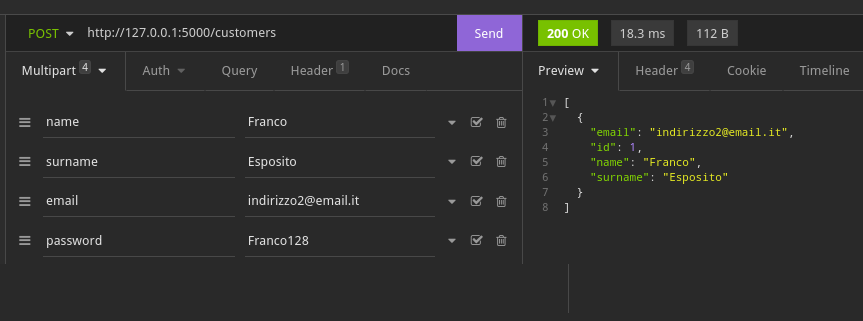
\includegraphics[scale=0.33]{images/inserimento_cliente.png}
\end{center}
\subsection{Inserimento categoria}

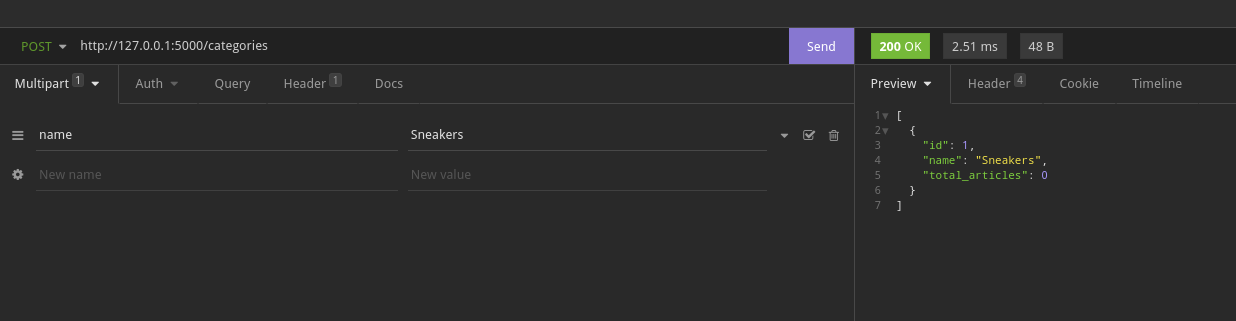
\includegraphics[scale=0.33]{images/inserimento_categoria.png}

\subsection{Inserimento prodotto}

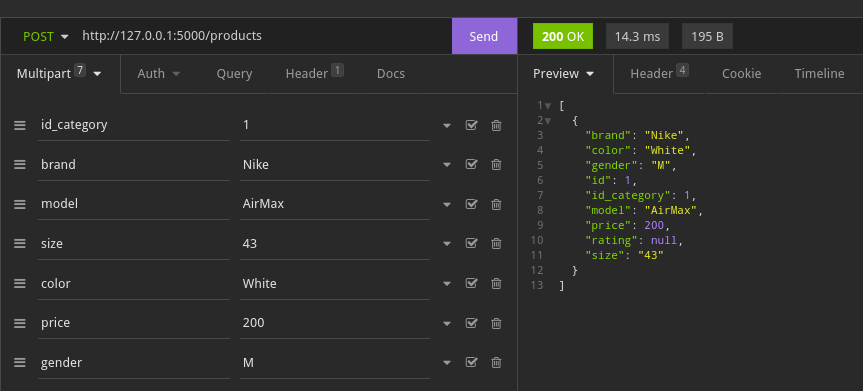
\includegraphics[scale=0.33]{images/inserimento_prodotto.png}

\subsection{Inserimento dipendente}

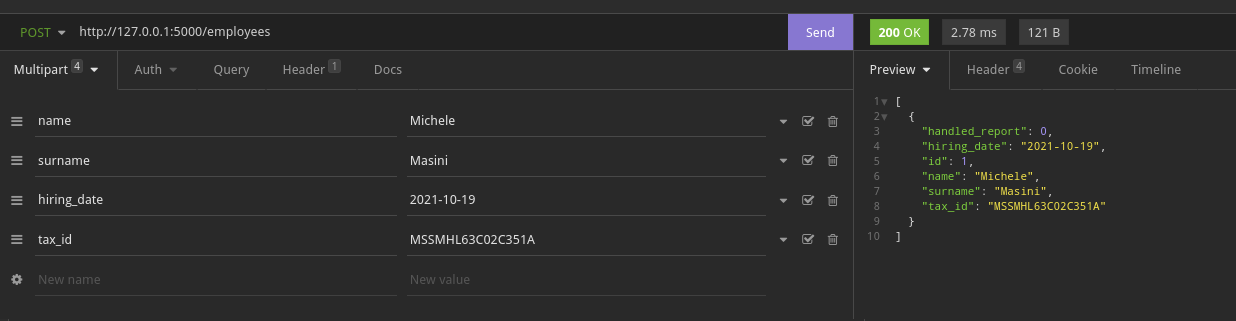
\includegraphics[scale=0.33]{images/inserimento_dipendente.png}

\subsection{Inserimento ordine}
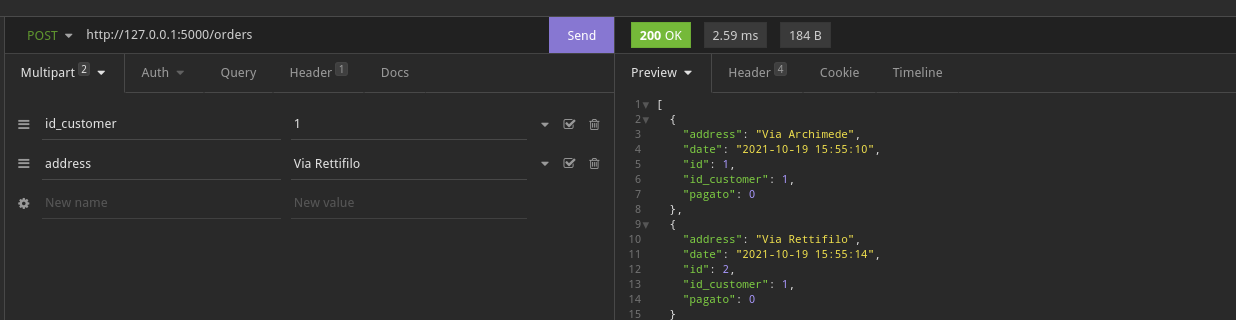
\includegraphics[scale=0.33]{images/ordine.png}

\subsection{Inserimento contenuto di un ordine}

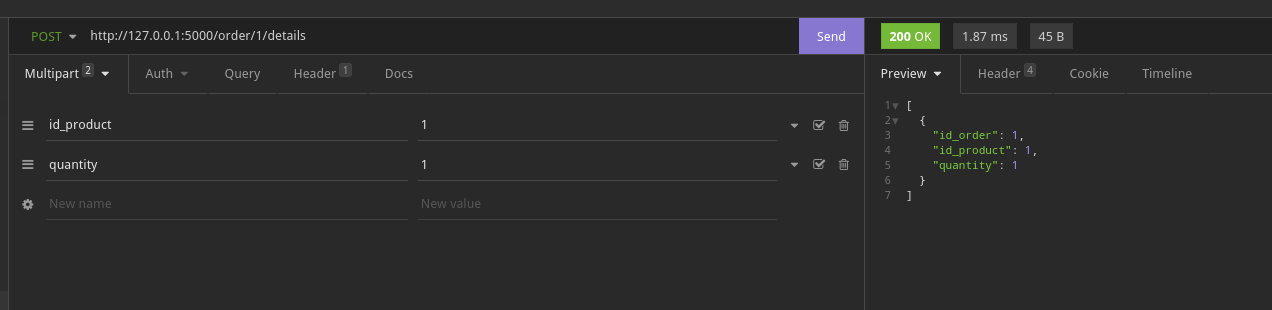
\includegraphics[scale=0.33]{images/inserimento_contenuto.png}

\subsection{Inserimento di uno sconto}

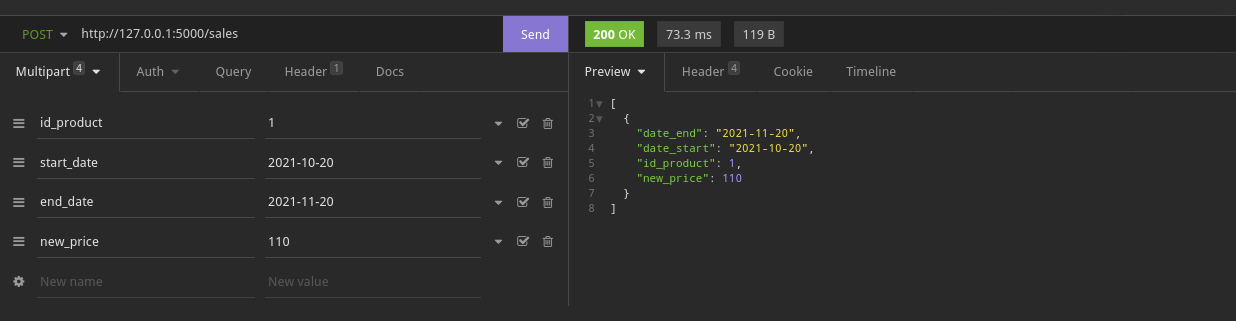
\includegraphics[scale=0.33]{images/inserimento_sconto.png}

\subsection{Pagamento ordine}

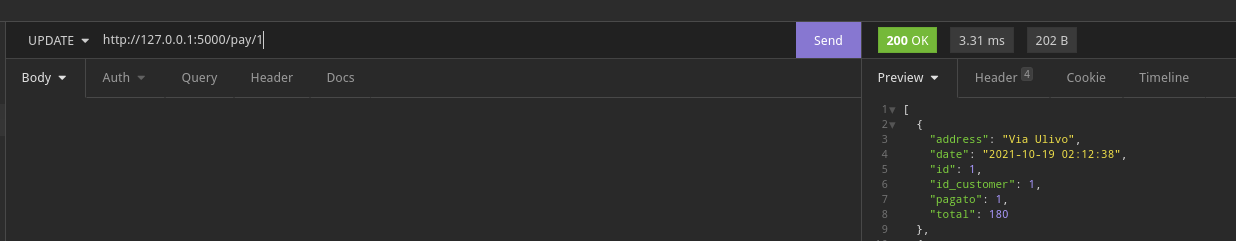
\includegraphics[scale=0.33]{images/ordine_pagato.png}

\subsection{Apertura segnalazione}

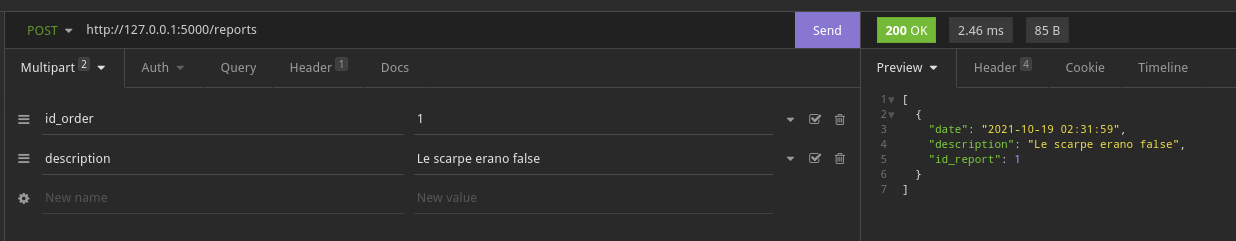
\includegraphics[scale=0.33]{images/inserimento_segnalazione.png}

\subsection{Chiusura segnalazione}

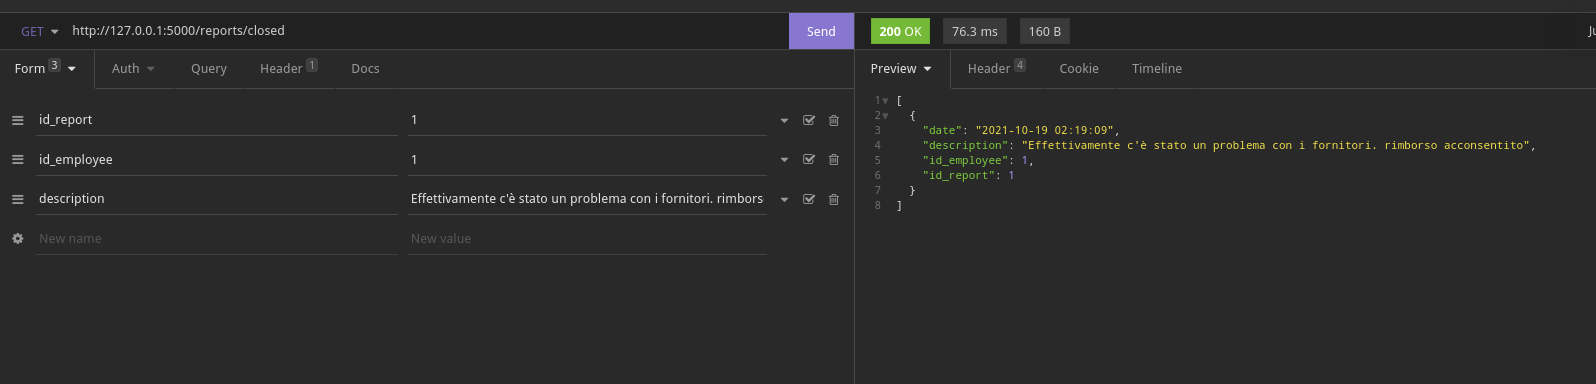
\includegraphics[scale=0.33]{images/chiusura_segnalazione.png}

\subsection{Rimborso concesso}

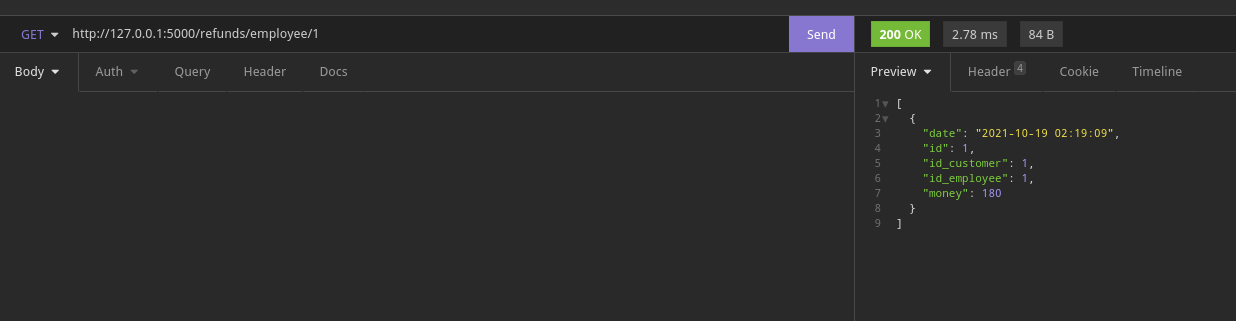
\includegraphics[scale=0.33]{images/rimborso.png}

\subsection{Inserimento di una recensione relativa a un prodotto}

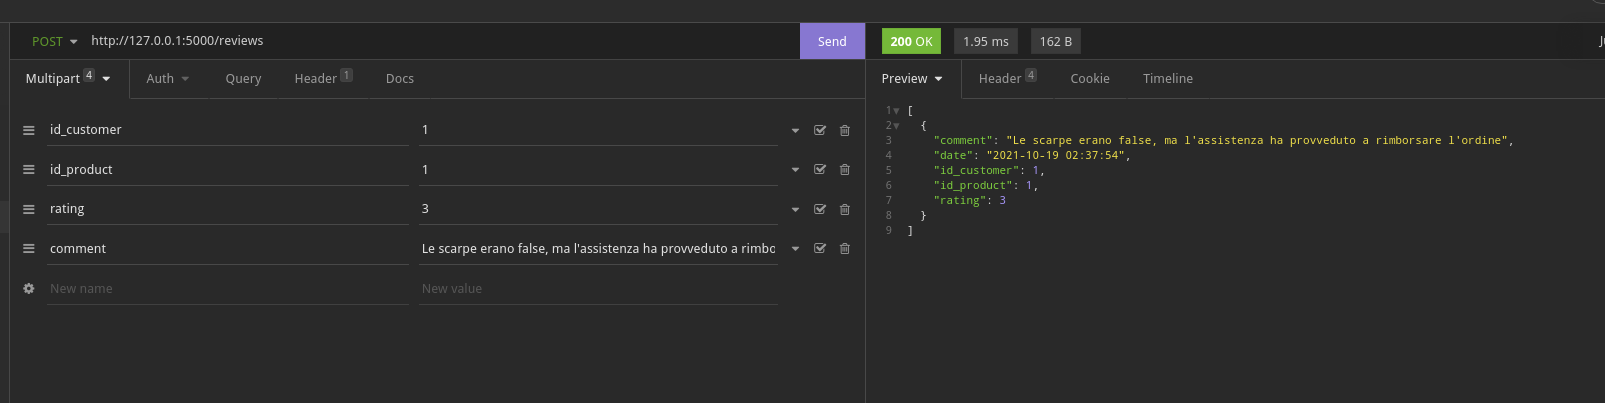
\includegraphics[scale=0.33]{images/recensione.png}

